\documentclass[letter,11pt]{article}
\usepackage[margin=1.5cm]{geometry}
\usepackage{latexsym}
\usepackage{amsmath}
\usepackage{color}
\usepackage{graphicx}
\usepackage{amssymb}
\usepackage{alltt}
\usepackage{enumitem}
\usepackage{siunitx}
\usepackage{physics}

\newenvironment{solution}{
    \vspace{0.16in} {\bf Solution:}
    
}{
	\vspace{0.16in}
}
\newcommand{\inti}[4]{
	\int_{#1}^{#2} #3 \, \mathrm{d} #4
}
\newcommand{\intii}[7]{
	\int_{#1}^{#2} \int_{#3}^{#4} #5 \, \mathrm{d} #6 \, \mathrm{d} #7
}
\newcommand{\expected}[1]{
    \mathbb{E}[#1]
}

%------------------------------------------------------

\begin{document}

\begin{center}
    {\bf \Large Math 189R problem set 1} \\
    \vspace{0.1in}
    Adam Guo \quad 2020-02-03
\end{center}

\begin{enumerate}
    \item {\bf (Linear Transformation)} Let ${\bf y} = A{\bf x} + {\bf b}$ be a random vector. Show that the expectation is linear: \[\mathbb{E}[y] = \mathbb{E}[A {\bf x} + {\bf b}] = A\mathbb{E}[{\bf x}] + {\bf b}\] Also show that \[cov[{\bf y}] = cov[A{\bf x} + {\bf b}] = A cov[{\bf x}] A^T = A \Sigma A^T\]

    \begin{solution}
        $\begin{aligned}
            \mathbb{E}[y] &= \inti{C}{}{(A{\bf x} + {\bf b}) Pr(x)}{x} \\
                &= \inti{C}{}{A{\bf x} Pr(x)}{x} + \inti{C}{}{{\bf b} Pr(x)}{x} & \quad \text{by linearity of integration} \\
                &= A \inti{C}{}{{\bf x} Pr(x)}{x} + {\bf b} \inti{C}{}{Pr(x)}{x} \\
                &= A \mathbb{E}[{\bf x}] + {\bf b}
        \end{aligned}$

        \vspace{0.16in}

        $\begin{aligned}
            cov[{\bf y}] &= \mathbb{E}[({\bf y} - \mathbb{E}[{\bf y}])({\bf y} - \mathbb{E}[{\bf y}])^T] \\
                &= \mathbb{E}[(A{\bf x} + {\bf b} - \mathbb{E}[A{\bf x} + {\bf b}])(A{\bf x} + {\bf b} - \mathbb{E}[A{\bf x} + {\bf b}])^T] \\
                &= \mathbb{E}[(A{\bf x} + {\bf b} - A\mathbb{E}[{\bf x}] - {\bf b})(A{\bf x} + {\bf b} - A\mathbb{E}[{\bf x}] - {\bf b})^T] \\
                &= \mathbb{E}[(A({\bf x} - \mathbb{E}[{\bf x}]))(A({\bf x} - \mathbb{E}[{\bf x}]))^T] \\
                &= \expected{A({\bf x} - \expected{{\bf x}})({\bf x} - \expected{{\bf x}})^T A^T} \\
                &= A \expected{({\bf x} - \expected{{\bf x}})({\bf x} - \expected{{\bf x}})^T} A^T \\
                &= A cov[\textbf{x}] A^T \\
                &= A \Sigma A^T, \quad \Sigma \equiv cov[\textbf{x}]
        \end{aligned}$
    \end{solution}

    \newpage

    %----------------------------------

    \item Given the dataset $\mathcal{D} = \{(x, y) = \{(0, 1), (2, 3), (3, 6), (4, 8)\}\}$,

    \begin{enumerate}
        \item Find the least squares estimate $y = \theta^T {\bf x}$ by hand using Cramer's Rule.

        \begin{solution}
            Let $\textbf{y} = \begin{bmatrix} 1 \\ 3 \\ 6 \\ 8 \end{bmatrix}, \quad \textbf{X} = \begin{bmatrix} 1 & 0 \\ 1 & 2 \\ 1 & 3 \\ 1 & 4 \end{bmatrix}$.
            
            By normal equations, $\textbf{X}^T \textbf{X} \hat{\theta} = \textbf{X}^T \textbf{y}$ such that $\hat{\theta}$ is the least squares estimate of $\theta$.

            $\textbf{X}^T \textbf{X} = \begin{bmatrix} 4 & 9 \\ 9 & 29 \end{bmatrix}, \quad \textbf{X}^T \textbf{y} = \begin{bmatrix}
                18 \\ 56
            \end{bmatrix}$

            Using Cramer's rule,

            $\displaystyle \hat{\theta}_1 = \frac{\begin{vmatrix} 18 & 9 \\ 56 & 29 \end{vmatrix}}{\begin{vmatrix} 4 & 9 \\ 9 & 29 \end{vmatrix}} = \frac{18}{35}, \quad \hat{\theta}_2 = \frac{\begin{vmatrix} 4 & 18 \\ 9 & 56 \end{vmatrix}}{\begin{vmatrix} 4 & 9 \\ 9 & 29 \end{vmatrix}} = \frac{62}{35}$
            
            Hence, $\hat{\theta} = \begin{bmatrix}
                \frac{18}{35} & \frac{62}{35}
            \end{bmatrix}$.
        \end{solution}

        \item Use the normal equations to find the same solution and verify it is the same as part (a).

        \begin{solution}
            $\begin{aligned}
                \theta &= (\textbf{X}^T \textbf{X})^{-1} \textbf{X}^T \textbf{y} \\
                    &= \begin{bmatrix} 4 & 9 \\ 9 & 29 \end{bmatrix}^{-1} \begin{bmatrix} 1 & 1 & 1 & 1 \\ 0 & 2 & 3 & 4 \end{bmatrix} \begin{bmatrix} 1 \\ 3 \\ 6 \\ 8 \end{bmatrix} \\
                    &= \frac{1}{35} \begin{bmatrix} 29 & -9 \\ -9 & 4 \end{bmatrix} \begin{bmatrix} 18 \\ 56 \end{bmatrix} \\
                    &= \frac{1}{35} \begin{bmatrix} 18 \\ 62 \end{bmatrix} \\
                    &= \begin{bmatrix} 18/35 \\ 62/35 \end{bmatrix}
            \end{aligned}$

            Same solution as part a.
        \end{solution}

        \item Plot the data and the optimal linear fit you found.

        \begin{solution}
            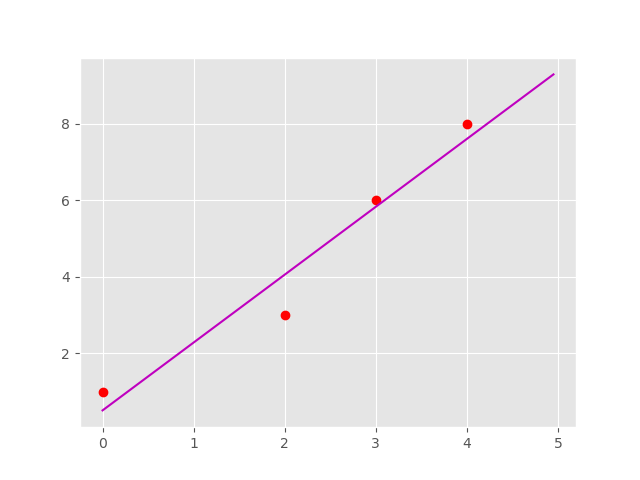
\includegraphics[width=12cm]{hw1pr2c.png}
        \end{solution}

        \item Find randomly generate 100 points near the line with white Gaussian noise and then compute the least squares estimate (using a computer). Verify that this new line is close to the original and plot the new dataset, the old line, and the new line.

        \begin{solution}
            The lines are very close.

            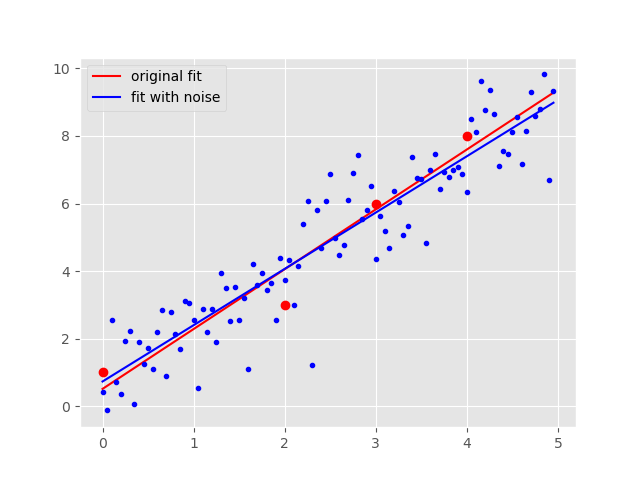
\includegraphics[width=12cm]{hw1pr2d.png}
        \end{solution}
    \end{enumerate}
\end{enumerate}

\end{document}